\chapter{Planning}

The smart home model box's development and planning began during Project Laboratory and has continued since then with some variations, including the replacement of software platform. This chapter takes a look at the planning work, before the plans were put into practice.

\section{General goals, requirements and principals of the planned model}

The box project's goal was to get familiar with the most important IoT and related technologies, such as microcontrollers, networking and electronics control and to put this knowledge into practice via the creation of a smart home model system demo box, which can then be used to gain experience with the usage of such a smart home or home automation system's evaluation.

During the box model project's planning and implementation phases, gaining a deeper insight of the underlying technologies and building a smart house solution from inexpensive, easy-to-obtain generic electronic components, microcontrollers and open-source software were favored over expensive, locked down out-of-the box solutions, as they are tuned for a quick and optimal end-user experience, but hide the implementation complexity from their users, therefore are less suitable for the project. The utilized software platform should be self-hosted in order to ensure absolute ownership of data and mitigate the vulnerability of being exposed to an external provider.

When finished, the box model should have electric and electronic devices inside it, which resemble utilities, that can be controlled along with sensors, detectors that collect the momentary status of different natural aspects at a given interval. It should also have a user interface, which can be used to control the appliances, display the current and historic readings of sensors accessible from a web browser or smartphone.

\section{Hardware environment}

The box containing the project's internals was chosen to be a shoebox, which I already had at hand and and is large enough to have separated rooms and smaller electric and electronic components inside it, but is also small enough to be easily transported. The floorplan of the house wasn't fixed at the planning phase due to the uncertainty of the picked devices' sizes, it was structured later in the implementation phase with cardboard to have separate rooms.

As for electronics inside the box, I decided on a single microcontroller board setup, where it is used to either control or read input from the connected devices and communicate to a server, which maintains all devices' status and provides a user interface. A microcontroller board is essentially a small computer, which is designed in a way to manage specific tasks within an embedded system without requiring a complex operating system. \cite{IBMmicrocontroller} Microcontrollers are well-suited for applications requiring real-time signal processing, such as controlling motors and servos and interfacing with various types of sensors and communications, therefore a great platform for home automation applications. The major microcontroller platforms considered for the project were Arduino, ESP and STM32. During Training Project Laboratory, I had the opportunity to use a NodeMCU ESP32S microcontroller, which is based on the ESP32S chip, that besides having a typical microcontroller functionality (ADC and DAC, PWM, UART and many more via their pins), also has wireless communication capabilities via Bluetooth and Wi-Fi. Due to this extra functionality often not being integrated in other microcontrollers, the cheap price and better price-to-value ratio, as well as the previous experience and easy access, I chose an ESP32-based NodeMCU ESP32S microcontroller board for the project. \cite{ESPvArduino} \cite{ESPvSTM}

One speciality of the selected NodeMCU microcontroller is its form factor, it has downward facing male pins, that can be plugged into a standard breadboard for easy connection to other electronics via jumper cables. Therefore many jumper cables and two breadboards were also obtained for the project, one breadboard for the microcontroller and one for higher powered device powering circuitry featuring transistors, because the microcontroller has a specified current limit on its pins, therefore wouldn't be able to provide enough power for certain components.

\begin{figure}[!ht]
    \centering
    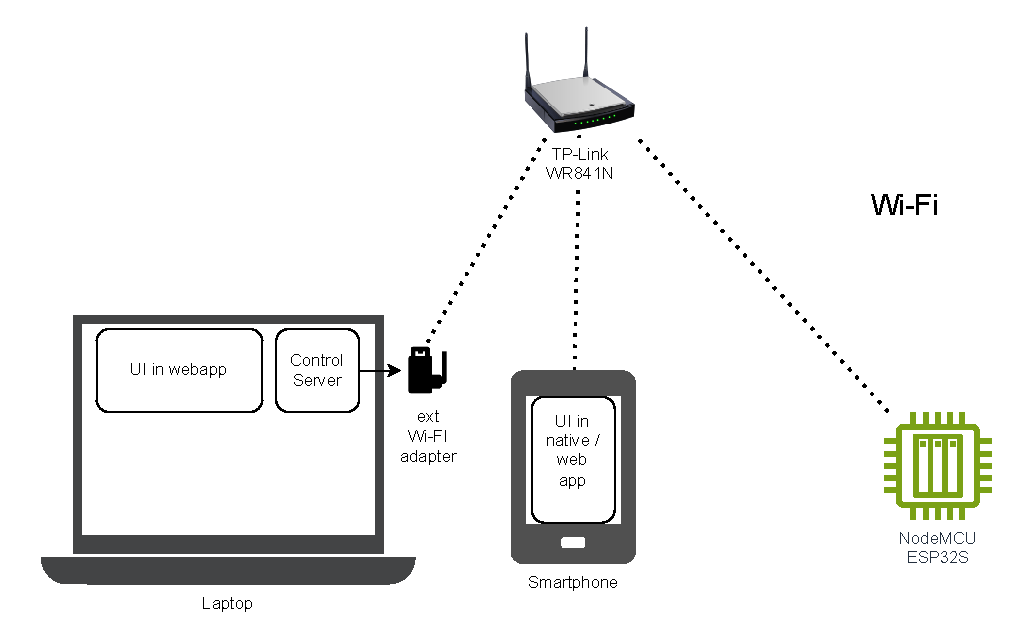
\includegraphics[page=1,keepaspectratio,width=150mm]{figures/box_network.drawio.pdf}
    \caption{Model network architecture}
    \label{fig:BoxNetwork}
\end{figure}

The communication medium between devices was chosen to be Wi-Fi, as this is one of the wireless protocols supported by microcontroller and by most laptops and smartphones, therefore a good common ground across devices. The control server was planned to be run on my own personal laptop for convenience and ease of development. Throughout Project Laboratory, I used a TP-Link WR841N at hand, which is a combined network device with routing, switching and Wi-Fi AP capabilities to symbolize a home network and provide a Wi-Fi network medium between devices. This remained in the the Thesis Project, with a custom firmware (DD-WRT) installed on it for more settings customization options, along with an extra Wi-Fi adapter plugged into the laptop for simultaneous usage of its internal Wi-Fi adapter to have Internet access. On \refstruc{fig:BoxNetwork}, a diagram of this network setup is shown.

One of the easily obtainable and connectable, yet spectacular electronic component that can be used in such a project is a Light Emitting Diode, or LED in short. A few LEDs and required resistors were obtained for the project in order to illuminate the rooms in a spectacular way, switched on or off from the user interface. Resistors of different common values were obtained to limit the current passing through components to protect them from overheating, for other devices as well, such as a light sensor in the form of an LDR (Light Dependent Resistor) and three LM235Z temperature sensors. For heating and cooling simulation, two 5V fans and a TEC1-12703 Peltier module were acquired. Two lower current rated BS170 transistors, two diodes and one higher current rated BD241C transistor were obtained for powering the two fans and the Peltier module from a high-current (2A) external 5V power supply (from a USB phone charger). And finally, an SG90 servo was acquired and fitted with extra parts to simulate an automated electronic rolling shutter.

\section{Software environment}

At the end of Project Laboratory, the software architecture of the model box was comprised of three main components: a JavaScript backend responsible for maintaining the components' status and communication between the microcontroller and user, microcontroller code for controlling the electronic components (reading sensor data, setting output for actuators), receiving and sending data to the backend and finally a React-based frontend to send commands and receive readings to and from the backend. For the Thesis Project, I decided to replace it with already available open-source smart home system platforms with more functionalities and better device and community support, because I believe it would have been harder to further develop it in an extensible way, add more features and the integration itself was also a great technical challenge to be featured as a Thesis Project.

Choosing the right smart home software platform for the project is an essential task, because it is the foundation of the project and the other subsystems depend on it. Its features and offers, hardware and software support, community reception should be considered before fully commiting to it, because changing to a different one can be tedious work if it doesn't meet the set requirements. After researching the major open-source smart home software platforms on the Internet, two projects were considered: Home Assistant and OpenHAB. \cite{HAHomepage} \cite{openHABHomepage} Both projects have mostly the same to offer for a smart home platform: both are open-source, have good documentation, have built-in UI with customizations and integrations for many kinds of devices and options for automations. However, Home Assistant has a larger community of users, contributors and its popularity is also bigger (a Google Trends comparison also confirms this). \cite{WunderTechHAvsopenHAB} With these findings and recommendation from acquaintances in mind, Home Assistant was chosen to be the base smart home platform.

The microcontroller software platform is also important for the success of the project, it has to be compatible with the smart home platform, be stable and has to have support for required device types and automations. Platforms compatible with Home Assistant for the ESP32S architecture were searched for and two major projects were found: ESPHome and Tasmota. Both focus primarily on supporting ESP-based microcontrollers, have integration for Home Assistant, mostly have the same popularity and community support and have support for Over-the-Air (OTA) updates. \cite{ESPHomeHomepage} \cite{TasmotaHomepage} \cite{ESPHomeOTA} \cite{TasmotaOTA} The main difference between the two projects are the technologies used for transmitting messages between the control server and microcontroller: ESPHome mainly uses Event Source API, but also has support for a simpler REST API and Tasmota uses MQTT, a message queueing protocol. \cite{ESPHomeWebAPI} \cite{TasmotaMQTT} Both use JSON payloads for their messages, however the technologies used by ESPHome usually make the propagation of control and other messages faster than Tasmota. Eventually, the microcontroller software platform was chosen to be ESPHome.
% maybe esphome yaml files here, or in impl?
